Hasta ahora hemos visto una idea general de las líneas de campo eléctrico. Es decir, vimos una explicación que busca dar una idea general de cómo funcionan las líneas de campo eléctrico, su forma, su dirección y su relación con las cargas, pero sin proporcionar fórmulas o cantidades específicas. En este apartado, vamos a explicar con mayor formalidad este concepto, donde se considerará la magnitud del campo eléctrico y el área a través de la cual se mide el flujo eléctrico, utilizando la relación matemática entre estas variables.

\subsubsection{Definición}

El \hl{flujo eléctrico} es una medida de la cantidad de campo eléctrico que atraviesa una superficie dada. Se define matemáticamente como el producto de la magnitud del campo eléctrico (\(E\)) y el área (\(A\)) de la superficie a través de la cual se mide el flujo, así como el coseno del ángulo (\(\theta\)) entre la dirección del campo eléctrico y la normal (perpendicular) a la superficie. La fórmula para calcular el flujo eléctrico (\(\Phi_E\)) es:

\begin{figure}[ht!]
    \centering
    \begin{subfigure}[b]{0.45\textwidth}
        \centering
        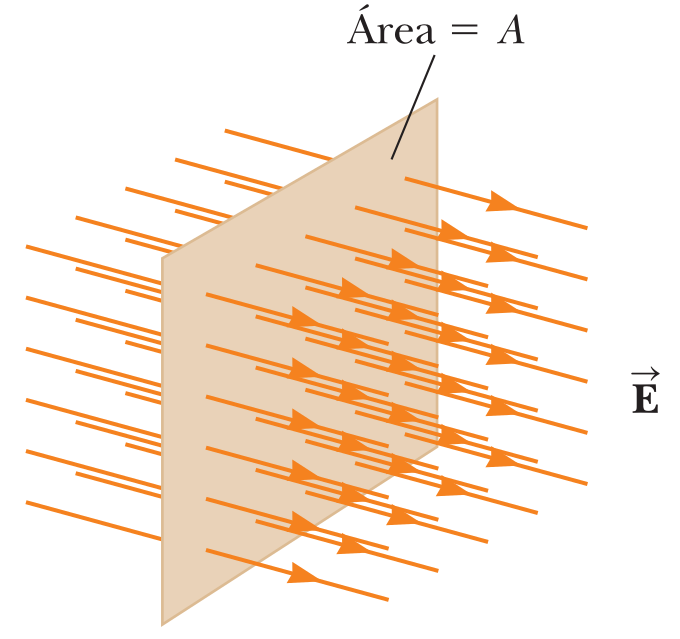
\includegraphics[width=\textwidth]{flujo_1.png}
        \caption{flujo sobre un area perpendicular.}
        \label{fig:flujo1}
    \end{subfigure}
    \hfill
    \begin{subfigure}[b]{0.45\textwidth}
        \centering
        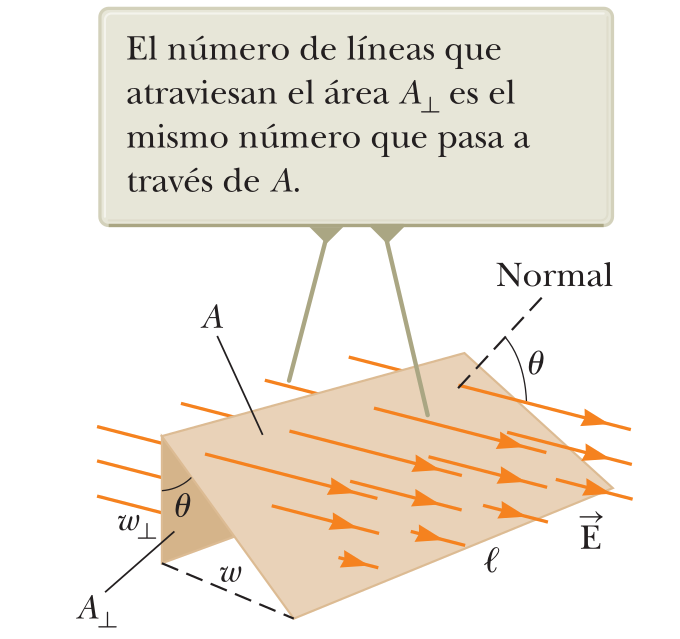
\includegraphics[width=\textwidth]{flujo_2.png}
        \caption{flujo sobre un area inclinada.}
        \label{fig:flujo2}
    \end{subfigure}
    \caption{Flujo eléctrico}
    \label{fig:flujo eléctrico}
\end{figure}

\[
\Phi_E = E \cdot A \cdot \cos(\theta)  ~~ \left[\frac{\si{\newton \meter \squared}}{\si{\coulomb}}\right]
\]

Donde:
\begin{itemize}
    \item \(\Phi_E\) es el flujo eléctrico.
    \item \(E\) es la magnitud del campo eléctrico.
    \item \(A\) es el área de la superficie.
    \item \(\theta\) es el ángulo entre la dirección del campo eléctrico y la normal a la superficie.
\end{itemize}

Otra forma más general de escribir el flujo eléctrico es usando el \hl{producto escalar}. Para poder usar el producto escalar, necesitamos dos vectores, y en este caso solo tenemos el vector de campo. Entonce podemos definir un vector normal a la superficie con igual magnitud al área de la superficie. Entonces el producto escalar entre el vector campo eléctrico (\(\vec{E}\)) y el vector normal al area \(\vec{A}\) es:

\begin{equation}
    \Phi_E = \vec{E} \cdot \vec{A} = E A \cos \theta
    \label{eq:flujo_electrico}
\end{equation}

Hay que tener muy presente que \(\Phi_E\) es un \textbf{ESCALAR} no un vector. Y otro factor a considerar es que la ecuación \eqref{eq:flujo_electrico} solo se puede usar si el campo \(\vec{E}\) es constante. Sin embargo, en general, el campo \(\vec{E}\) no suele ser constante, entonces una forma de conseguir el flujo eléctrico total en una superficie \(S\) donde el campo no es constante es sumando todas las pequeñas contribuciones de flujo eléctrico en pequeñas porciones de area (\(dA\)), resultando en la siguiente integral:

\begin{equation}
    \Phi_E = \int_{S} \vec{E} \cdot d\vec{A}
    \label{eq:flujo_electrico_integral}
\end{equation}

\subsubsection{Ley de Gauss}

El flujo eléctrico es importante en el estudio del electromagnetismo porque está relacionado con la ley de Gauss, que establece que el flujo eléctrico a través de una superficie \textbf{cerrada} (con frecuencia llamada \textit{superficie gaussiana}) es proporcional a la carga eléctrica total encerrada dentro de esa superficie.

\begin{wrapfigure}{r}{0.35\textwidth}
    \centering
    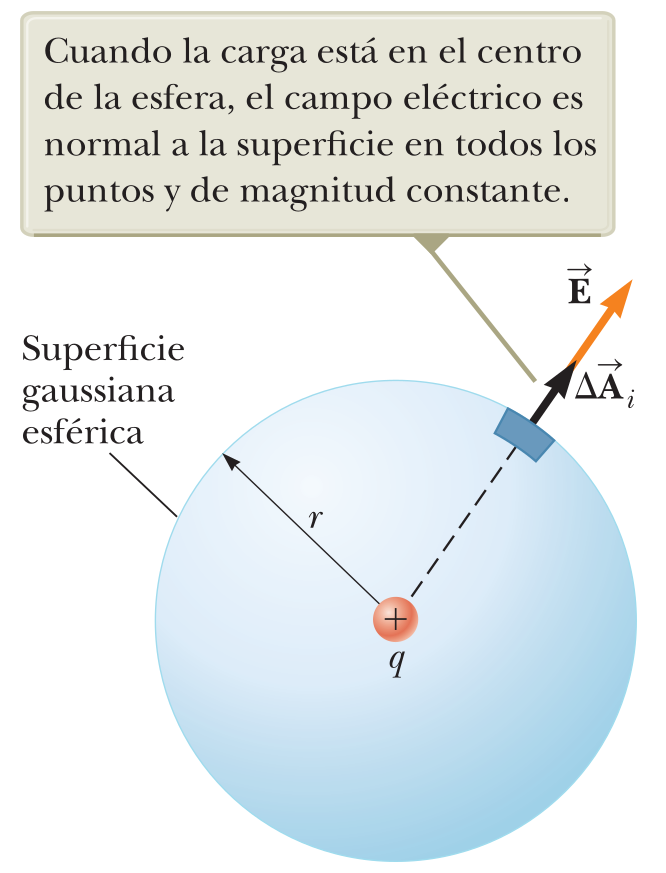
\includegraphics[width=0.33\textwidth]{ley_de_gauss.png}
    \caption{Superficie gaussiana esférica de radio \(r\) que rodea una carga puntual \(q\).}
    \label{fig:superficie_gaussiana}
\end{wrapfigure}

Suponga una carga puntual positiva \(q\) ubicada en el centro de una esfera de radio \(r\) como se observa en la figura \ref{fig:superficie_gaussiana}. De la ecuación de campo eléctrico \eqref{eq:campo_electrico}, se sabe que la magnitud del campo eléctrico sobre todos los puntos de la superficie (\(S\)) de la esfera es \(\vec{E} = k q/r^2\). Las líneas de campo están dirigidas radialmente hacia afuera y por tanto son perpendiculares a la superficie en todos sus puntos. Es decir, en cada punto de la superficie, \(\vec{E}\) es paralelo al vector \(d\vec{A}\) que representa un elemento de área muy pequeño que rodea al punto en la superficie. Por lo tanto, el flujo neto a través de la superficie gaussiana es igual a:

\begin{align*}
    \Phi_E =& \oint_S \vec{E} \cdot d\vec{A} \\
            =& \oint_S E \cos(0) ~ dA \\
            =& \oint_S E ~ dA \\
    \Phi_E =& E ~ \oint_S dA
\end{align*}

aquí tenemos que \(E=kq/r^2\) donde \(r\) es conocido y vale el radio de la esfera, \(q\) es el valor de la carga en el centro de la esfera y \(k = 1/4\pi\epsilon_0\). Luego la integral resulta en la superficie de una esfera que es \(4\pi r^2\). Entonces:

\[
\Phi_E = E ~ \oint_S dA = \frac{q}{4\pi \epsilon_0 r^2} \cdot 4\pi r^2 = \boxed{\frac{q}{\epsilon_0}} 
\]

Este resultado dice muchas cosas:
\begin{itemize}
    \item \textbf{Primero}: el flujo eléctrico \(\Phi_E\) no depende del radio de la superficie esférica.
    \item \textbf{Segundo}: el flujo es directamente proporcional a la carga encerrada en el interior de la superficie gaussiana.
    \item \textbf{Tercero}: el flujo es inversamente proporcional al valor de \(\epsilon\), en el ejemplo se tabajó con vacío, pero puede ser cualquier material no conductor con otro valor de \(\epsilon\).
\end{itemize}

En base a esto podemos sacar una conclusión, supongamos ahora que la superficie no es esférica ¿El flujo será el mismo que el de la esfera? Bueno, pues voy a hacer un adelanto, si lo es, pero ¿Por qué? Pensemos en la definición de flujo, sea cualquier superficie que rodea la esfera, el flujo será igual a el \(\vec{E}\cdot d\vec{A}\). Como vimos anteriormente esto representa la cantidad de líneas de campo que pasan por una superficie determinada. Como la superficie encierra la misma carga entonces saldrán la misma cantidad de líneas de campo por la superficie.

En este punto tal vez te preguntes ¿Cómo puede ser que no dependa del radio de la esfera, o mejor del tamaño de la superficie arbitraria cerrada? Es sencillo, si el tamaño de la superficie cerrada aumenta, entonces la distancia a la carga encerrada también aumentará, esto significa que la intensidad del campo disminuirá, entonces pasarán menos líneas de campo por cada \(dA\), pero como la superficie total a aumentado, entonces compensará la pérdida de intensidad del campo.

Con esto podemos armar una conclusión:

\begin{tcolorbox}[myconclusion]
    el flujo neto a través de \textit{cualquier} superficie cerrada que rodea a una carga puntual \(q\) está dado por \(q/\epsilon_0\) y es independiente de la forma de la superficie.
\end{tcolorbox}

Entonces, si suponemos varias superficies, llamemos \(S1\), \(S2\) y \(S3\) a las superficies que rodean la carga \(q\) (ver figura \ref{fig:superficie_gaussiana_arbitraria}). Todas estas superficies tienen el mismo flujo eléctrico, ya que todas encierran la misma carga \(q\). Se puede ver que el flujo neto es el mismo para todas las superficies.

\begin{figure}[ht]
    \centering
    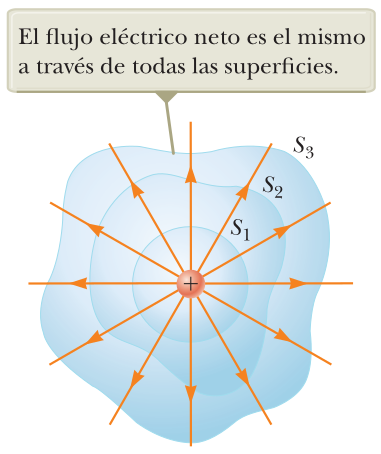
\includegraphics[width=0.35\textwidth]{flujo_neto.png}
    \caption{Distintas superficies gaussianas de forma arbitraria que rodean una carga puntual \(q\).}
    \label{fig:superficie_gaussiana_arbitraria}
\end{figure}

Por otro lado, si la carga \(q\) está fuera de la superficie gaussiana entonces la misma cantidad de líneas de campo que entran por un lado de la superficie, salen por el otro lado. Por lo tanto, el flujo neto a través de la superficie es cero. Esto se puede ver en la figura \ref{fig:flujo_neto_2} donde se observa que el flujo neto es cero.

\begin{figure}[ht]
    \centering
    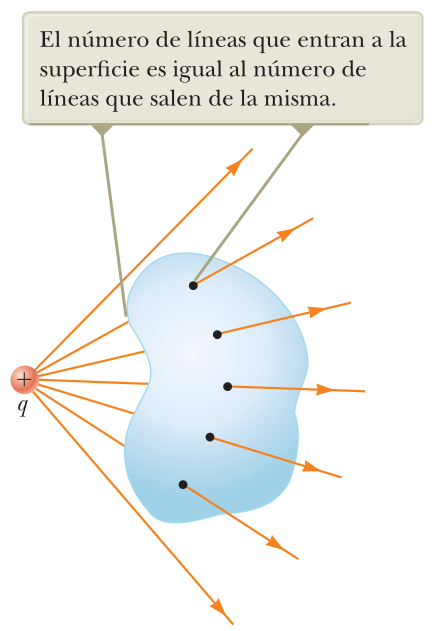
\includegraphics[width=0.4\textwidth]{flujo_neto_externo.png}
    \caption{Una carga puntual \(q\) fuera de la superficie.}
    \label{fig:flujo_neto_2}
\end{figure}

La forma matemática de ley de Gauss, es una generalización de lo anterior y establece que el flujo neto a través de cualquier superficie cerrada es

\begin{equation}
    \Phi_E = \oint_{S} \vec{E} \cdot d\vec{A} = \frac{q_{\text{int}}}{\varepsilon_0} ~~ \left[\frac{\si{\newton \meter \squared}}{\si{\coulomb}}\right]
\end{equation}

donde:
\begin{itemize}
    \item \( \Phi_E \) es el flujo de campo eléctrico a través de una superficie cerrada.
    \item \(E\) es el campo eléctrico en cada punto de esa superficie.
    \item \(dA\) es un vector diferencial de área que apunta hacia afuera de la superficie.
    \item \(q_{int}\) es la carga total encerrada dentro de la superficie.
    \item \(\epsilon_0\) es la permitividad del vacío, una constante del medio.
\end{itemize}

\begin{tcolorbox}[mydanger]
    CUIDADO: \(\vec{E}\) representa el campo eléctrico total, que incluye contribuciones de ambas cargas tanto del interior como del exterior de la superficie.    
\end{tcolorbox}

\paragraph{¿Qué nos dice esta ley, en términos simples?}

El flujo eléctrico representa la cantidad de ``líneas de campo eléctrico'' que atraviesan una superficie. La ley de Gauss nos habla de superficies cerradas, y nos dice que si hay carga dentro de una superficie cerrada, el campo eléctrico ``sale'' (o ``entra'') por esa superficie, generando un flujo distinto de cero. Si no hay carga neta dentro, el flujo eléctrico total es cero, aunque el campo pueda no ser nulo en todos los puntos. No importa la forma de la superficie, solo importa cuánta carga encierra, no cómo se distribuye el campo en detalle.

\subparagraph{¿Por qué es útil la ley de Gauss?}

La ley de Gauss es útil porque, en situaciones con alta simetría (esférica, cilíndrica, planar), permite calcular el campo eléctrico sin integrar la ley de Coulomb, por ejemplo:
\begin{itemize}
    \item Una esfera cargada uniformemente
    \item Un hilo infinitamente largo con carga lineal uniforme
    \item Un plano infinito cargado
\end{itemize}

\subparagraph{Ejemplo clásico: esfera cargada}

Supón una carga distribuida uniformemente en una esfera. Si elegimos una superficie esférica de radio  mayor al de la esfera, por simetría:
\[
\vec{E} = \text{constante} \quad \text{y} \quad \vec{E} \parallel d\vec{A}
\]
Entonces la integral se simplifica:
\[
\oint \vec{E} \cdot d\vec{A} = E \oint dA = E(4\pi r^2)
\]
Y por la ley de Gauss:
\[
E(4\pi r^2) = \frac{Q}{\varepsilon_0} \quad \Rightarrow \quad E = \frac{1}{4\pi\varepsilon_0} \frac{Q}{r^2}
\]
¡Y así recuperamos la fórmula del campo eléctrico de una carga puntual!